\section{Proposed Method}
\label{sec:method}

\subsection{Query-Level Formulation and Overview}

Let $\mathcal X$ denote an annular weld image. The detector produces hypotheses $\{(b_i,q_i,z_i)\}$, where $b_i$, $q_i$, and $z_i$ are the bounding box, D-FINE-S query, and class-logit vector for candidate $i$, respectively. The relevant decision is not solely whether $z_i$ exceeds a global threshold. It is whether $q_i$ is supported by reliable local defect evidence. NORA therefore augments each query with a spatial evidence vector $\widehat E_i^s$ and a local-frequency evidence vector $\widehat E_i^f$. Their contributions are determined for each candidate rather than fixed over the dataset.

Figure~\ref{fig:cyclicibo} summarizes the forward path. Geometry-preserving cyclic windows provide local context. IBO regions convert a candidate into interior, boundary, and outside observations. A normal-reference bank converts raw transitions into position-conditioned deviations. The reliability-guided fusion block estimates the reliability of spatial and frequency deviations and preserves their disagreement when it is informative. Cyclic merging and restricted correction are post-fusion decision safeguards; they do not replace the fusion mechanism.

\begin{figure*}[t]
\centering
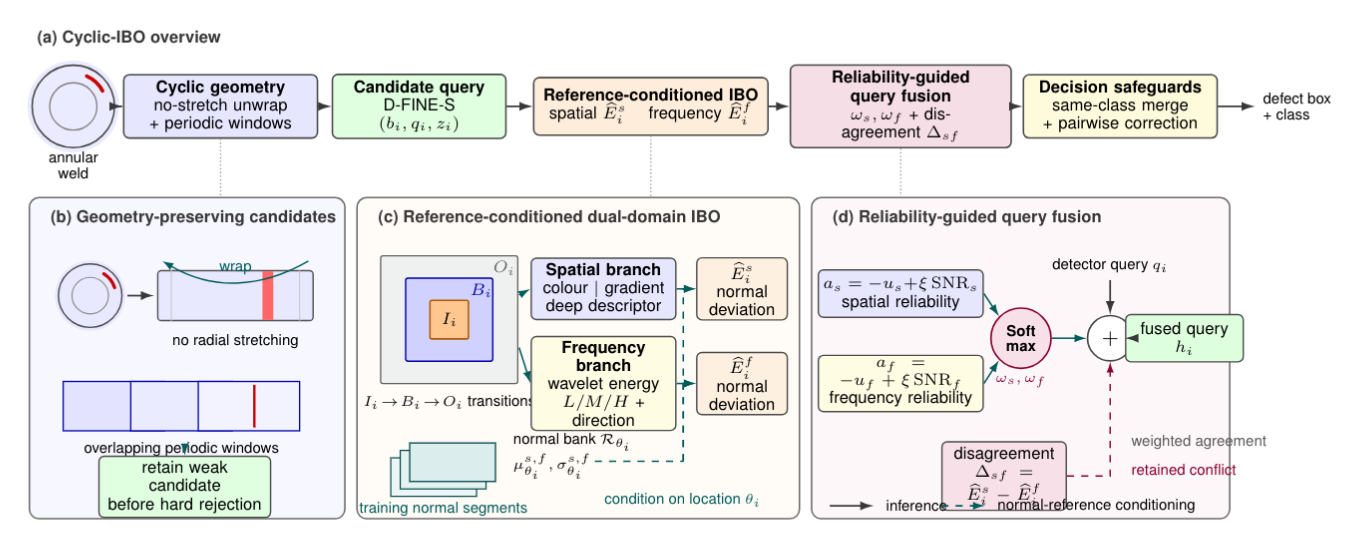
\includegraphics[width=\textwidth]{figures/fig1_cyclic_ibo_overview.png}
\caption{Overview of NORA. (a) The complete candidate--evidence--decision path. (b) No-stretch unwrapping and periodic windows preserve the closed seam while retaining weak detector candidates. (c) Spatial and local-frequency $I\!\rightarrow\!B\!\rightarrow\!O$ transitions are converted into deviations from normal segments at the same circumferential location. (d) Candidate-specific reliability weights combine the two domains while an explicit disagreement path retains diagnostic cross-domain conflict.}
\label{fig:cyclicibo}
\end{figure*}

\subsection{Geometry-Preserving Candidate Queries}

The annular seam band is unwrapped into a strip without radial stretching. It is not resized to force a curved region into a rectangular geometry. The strip is divided into overlapping windows of width 150 pixels. A window that crosses the artificial $0/2\pi$ seam origin is completed with pixels from the opposite end of the strip. This cyclic construction preserves local context for defects near the origin and avoids introducing a nonphysical boundary into the input.

Localization remains the detector's responsibility. NORA operates after a candidate query has been generated because spatial--frequency reasoning cannot recover a defect removed by geometric distortion or missing local context. The centre of candidate $i$ defines a circumferential location bin $\theta_i$. This bin retrieves comparable normal-seam statistics; it is not used as a class label.

\subsection{Normal-Reference IBO Transition Evidence}
\label{sec:ibo-evidence}

\textbf{IBO representation.} Candidate $i$ is decomposed into an interior $I_i$, a scale-adaptive boundary ring $B_i$, and an outside context ring $O_i$. The rings are clipped to the unwrapped seam band. The resulting representation captures two local transitions: from the candidate interior to its boundary and from that boundary to the neighbouring seam.

\textbf{Spatial transition.} From each region $r\in\{I,B,O\}$, we pool colour and luminance statistics $C_{i,r}$ in Lab space, gradient magnitude and orientation $G_{i,r}$, and a deep spatial descriptor $Z_{i,r}$ from the detector feature pyramid:
\begin{equation}
T_{i,r}^{s}=[C_{i,r},G_{i,r},Z_{i,r}].
\end{equation}
The spatial IBO transition is
\begin{equation}
E_i^{s}=[T_{i,B}^{s}-T_{i,I}^{s},\;T_{i,O}^{s}-T_{i,B}^{s}].
\label{eq:spatial-transition}
\end{equation}
It describes local structural change rather than an absolute colour or texture response.

\textbf{Local-frequency transition.} A whole-image Fourier transform does not reliably localize small defects when periodic metal texture dominates the response. We therefore compute a local multi-scale wavelet decomposition independently in $I_i$, $B_i$, and $O_i$. Let $A_{i,r}^{L,M,H}$ denote pooled low-, middle-, and high-frequency energies together with directional responses. The frequency transition is
\begin{equation}
E_i^{f}=[\log A_{i,B}-\log A_{i,I},\;\log A_{i,O}-\log A_{i,B}].
\label{eq:frequency-transition}
\end{equation}
The frequency branch thus evaluates a local spectral transition. It does not assume that greater high-frequency energy always indicates a defect.

\textbf{Normal-reference conditioning.} A reference bank stores $\mathcal R_{\theta}=\{\mu_{\theta}^{s},\sigma_{\theta}^{s},\mu_{\theta}^{f},\sigma_{\theta}^{f}\}$, estimated from verified normal seam segments at each location bin. Both transitions are standardized with the compatible reference:
\begin{equation}
\widehat E_i^d=\frac{E_i^d-\mu_{\theta_i}^d}{\sigma_{\theta_i}^d+\epsilon},\quad d\in\{s,f\}.
\label{eq:reference-conditioning}
\end{equation}
This operation reduces the ambiguity of absolute features. A reflection that routinely occurs at a location can be discounted, whereas a local departure from comparable normal seam remains salient. The candidate under assessment is not used to update its reference entry.

\subsection{Reliability-Guided Spatial--Frequency Query Fusion}
\label{sec:reliability-fusion}

Reliability-guided fusion is the central component of NORA. Fixed concatenation or summation assumes that the two domains are equally dependable. For each $d\in\{s,f\}$, we instead estimate a branch uncertainty $u_d$ and a reference-normalized anomaly strength $\mathrm{SNR}_d$. In the proposed fusion head, a lightweight predictor maps the evidence vector to $u_d\geq0$, and anomaly strength is defined as the normalized evidence magnitude:
\begin{equation}
\mathrm{SNR}_d=\frac{\|\widehat E_i^d\|_2}{\sqrt{\dim(\widehat E_i^d)}}.
\end{equation}
The reliability weights are
\begin{equation}
(\omega_s,\omega_f)=\operatorname{Softmax}(-u_s+\xi\,\mathrm{SNR}_s,\;-u_f+\xi\,\mathrm{SNR}_f),
\label{eq:reliability}
\end{equation}
where $\xi$ controls the contribution of reference-normalized anomaly strength. A branch receives more weight when it is both confident and anomalous relative to normal seam at the same location.

The fused query is
\begin{equation}
h_i=q_i+\omega_sW_s\widehat E_i^s+\omega_fW_f\widehat E_i^f+W_\Delta(\widehat E_i^s-\widehat E_i^f).
\label{eq:fusion}
\end{equation}
The last term does not enforce agreement. It retains diagnostic disagreement patterns. A reflection-like candidate can be spatially strong but spectrally unstable; a small pore can be frequency-dominant at its boundary; and a smoke-like change can be spatially or low-frequency dominant. Accordingly, $h_i$ encodes corroborating evidence and the form of conflict between the two domains. The classification head operates on $h_i$ rather than an unconditioned feature concatenation.

For an end-to-end instantiation, the detector loss is augmented with spatial, frequency, fused-query, and candidate-reliability objectives:
\begin{equation}
\mathcal L=\mathcal L_{\mathrm{D\text{-}FINE}}+\lambda_s\mathcal L_s+\lambda_f\mathcal L_f+\lambda_j\mathcal L_j+\lambda_r\mathcal L_{\mathrm{rel}}.
\label{eq:loss}
\end{equation}
Here, $\mathcal L_{\mathrm{D\text{-}FINE}}$ is the anchor detection objective and its coefficient is fixed to one. The coefficient $\lambda_s$ controls supervision of the spatial-transition branch; it prevents the branch from becoming a passive feature source, but avoids allowing illumination or reflection cues to dominate the detector. Likewise, $\lambda_f$ controls local-frequency supervision, retaining sensitivity to weak boundary and band-transition cues while limiting over-response to metal texture and acquisition noise. The coefficient $\lambda_j$ weights the discriminative objective on the fused query. It requires the combined representation to support the final decision, rather than collapsing to one branch, but does not force spatial and frequency evidence to agree. Finally, $\lambda_r$ weights candidate-reliability supervision. It calibrates the evidence gate so that uncertain or normal-reference-inconsistent evidence cannot dominate the decision; excessive reliability weighting would instead make the detector overly conservative for low-score tail candidates.

The coefficients balance auxiliary evidence learning against detector stability and are selected jointly on the validation set as
\begin{equation}
\max_{\lambda_s,\lambda_f,\lambda_j,\lambda_r,\,k}\; AP_T(k)
\quad\text{s.t.}\quad
AP_H(k)\geq AP_H^{\mathrm{base}}-\delta,
\label{eq:weight-selection}
\end{equation}
where $k$ denotes the checkpoint, $AP_T$ and $AP_H$ denote tail- and head-class AP, and $\delta$ is the permitted head-class reduction. This criterion selects evidence weights and a checkpoint for tail improvement without accepting an unconstrained loss of head-class performance.

\subsection{Decision Safeguards: Cyclic Merging and Restricted Correction}

Overlapping cyclic windows can generate several hypotheses for one physical defect. We merge only boxes with the \emph{same predicted class} across overlapping windows. No cross-class vote is permitted. This removes duplicate predictions without enabling a frequent class to absorb a weak tail class during merging.

A second global classifier would create additional opportunities for error across the full label space. We instead construct a confusion graph from held-out error audits and activate contrastive correction only for recurrent tail-to-head or visually similar pairs. Within an active pair, the candidate crop and fused query $h_i$ are compared with pair-specific prototypes. The correction may re-rank the pair but cannot propose a class outside the audited pair. This restricts the operation to observed confusions while preserving the detector's original decision space.
